\documentclass[10pt,a4paper,twoside]{book}
\usepackage[utf8]{inputenc}
\usepackage{amsmath}
\usepackage{amsfonts}
\usepackage{amssymb}
\usepackage{graphicx}
\usepackage{hyperref}
\usepackage{minted}
\usepackage[left=2cm,right=2cm,top=2cm,bottom=2cm]{geometry}
\newtheorem{mydef}{Theorem}

\makeindex

\begin{document}
\title{Bayesian optimization in machine learning}
\author{Jos\'e Jim\'enez Luna}
\maketitle
\tableofcontents


\chapter{Organization of this work}

\section{Introduction}

This master's thesis objective is to provide an easy to follow manual to users who want to use some form of Bayesian Optimization in practice. While the theory of Bayesian Optimization itself is pretty new, the foundations on which it is implemented in practice have been formally presented since the 90s. This work itself does not develop any new theory, but aims to provide users with both a theoretical and a practical introduction to Bayesian Optimization, as well as a Python implementation that users can use in their research.\\

Readers will find code during theoretical explanations, as I believe the easiest way to learn is to do. This will hopefully be beneficial for the reader. All the code implemented is available with a MIT license in a GitHub repository (\url{https://github.com/hawk31/pyGPGO}). This is a Python ($>$3.5) package that provides most of the functionality presented in this manual.\\

Bayesian Optimization focuses on the global optimization of a function $f:\mathbb{R}^n \rightarrow \mathbb{R}$ over a compact set $A$. The problem can be formalized as:

\begin{equation}
\max_{\boldsymbol{x}\in A} f(x)
\end{equation}

Most optimization procedures (local based ones such as gradient ascent, for example) assume that the function $f$ is closed-form, that is, can be written in a paper, that it is convex, with known first or second order derivatives or cheap to evaluate. Bayesian optimization focuses on all these problems proposing a very elegant solution. By the use of a surrogate model, a Gaussian Process, a Bayesian optimization procedure can help to find the global minimum of a non-necessarily convex, expensive functions. These methods shine also where there is no closed-form expression to evaluate and does not need any function derivatives.\\

Now is when the machine learning part of the title comes into play. In machine learning, we are usually interested in minimizing (or maximizing the opposite) a loss function $L$. These losses can take many forms, for example, when doing regression, a typical loss might be the mean squared error between predictions and observed values on a holdout test set.

\begin{equation}
L(\boldsymbol{y}, \boldsymbol{\hat{y}}) = \dfrac{1}{n} \sum_i \left(y_i - \hat{y_i}\right)^2
\end{equation}

In binary classification, for example, a very popular loss function example is the logarithmic loss:

\begin{equation}
L(\boldsymbol{y}, \boldsymbol{\hat{y}}) = -\dfrac{1}{n} = \sum_i \left(y_i \log(\hat{y_i}) + (1 - y_i)\log(1-\hat{y_i})\right)
\end{equation}

Focus in any case, that these losses are typically defined in a subset of $\mathbb{R}$. We focus on the supervised setting of machine learning, and more specifically regression. Depending on the problem at hand, even evaluating these losses can be very expensive from a computational point of view. This may have to do with the machine learning algorithm used or the size of the dataset at hand. These machine learning algorithms typically have \textit{hyperparameters}, that is, parameters that have to be tuned in a sensible way to get the best performance possible out of these models. In the machine learning community it is common for practitioners to do an hyperparameter grid search or even randomize it. Since the training of a single model can already take substantial resources in terms of CPU cycles or memory, we would like to have a more efficient and cheap way to optimize these hyperparameters. Bayesian optimization will let us do that by proposing the next candidate point $\boldsymbol{x}$ to evaluate according to several criteria.

\section{How this manual is supposed to be read}

Before we dive directly into the topic at hand, it is mandatory to explain how this manual is intended to be read. Different chapters will cover different material, so if the reader is familiar with a topic in a chapter, for example, the chapter on Gaussian Processes, he can skip directly to the chapter on Bayesian Optimization or to the implementation if he wishes. There is no complicated material in any of the chapters, as this manual does not aim to be research material on the the latest advances in the already quite crowded field.\\

\textbf{Chapter 2} focuses on a swift but thorough introduction to regression problems using Gaussian Processes. These are the surrogate models we will use for Bayesian Optimization in Chapter 3. We will cover the theory behind them both from a weight space view and from a functional view. We will also explain different covariance functions and their role in these models, as well as methods for optimizing their hyperparameters. Finally we will provide the reader with usable code to fit a Gaussian Process in a regression problem. This chapter is heavily based on Carl E. Rasmussen excellent book \textit{Gaussian Processes for Machine Learning}[ref]. In fact, if the reader is interested in a more advanced, wider, slowly-paced introduction to Gaussian Processes, this is the resource to go to. \\

\textbf{Chapter 3} is about the main topic in this work, Bayesian Optimization. Once we have laid down all the foundations of Gaussian Processes, we can start explaining the theory of Bayesian optimization using these as surrogate models. The algorithms, while simple, are very powerful. The role of several acquisition functions, that is to say, the functions that will propose the next point to evaluate will be discussed, as well as their advantages or disadvantages. The references on this chapter will be more diverse than on the previous chapter, as I will try to summarize several publications.\\

\textbf{Chapter 4} covers experiments using the software provided alongside this manual. These are mostly mid-sized regression or classification problems where we will compare the performance of Bayesian Optimization of hyperparameters with several regressors/classifiers with other strategies, such as random search or simulated annealing. Most of these datasets are related to experimental sciences, and some of them are typically used for other benchmarking purposes in other studies. Readers already familiar with Gaussian Processes should jump directly into this chapter.\\

\textbf{Chapter 5} is the shortest one. It will cover technical explanations of pyGPGO, the software developed alongside this manual. I will also try to provide practical examples on how to use the software.

\chapter{Gaussian Process regression}

We will focus on regression problems in this chapter. Assume we have some labelled data $D = \left\lbrace \left(\boldsymbol{x_i}, y_i\right) | i = 1,\dots,n\right\rbrace$, where $x$ is a vector of covariates and $y$ denotes a continuous objective variable. We wish to learn a predictive distribution over new values of $x$, so that we can make predictions and inference over these. In practice, for simplicity we write that $D = \left(X, \boldsymbol{y}\right)$, where $X$ is a covariate matrix.\\

One can interpret a Gaussian Process in several ways, the most used one is the function space view, which is the one we will cover second here and the one we will assume for the rest for the manual. In this view, we consider a Gaussian Process to be a distribution over functions, instead of over values. Inference takes place directly in this space. For completeness, we will also provide a weight-space view first, that might be more appealing to readers familiar with Bayesian linear regression.\\

\section{A weight space view for Gaussian Processes}

In this section we will try to draw connections between Bayesian linear regression and our introduction to Gaussian Processes, by the use of kernel functions. 

\subsection{Standard Bayesian linear regression}

A Bayesian linear regression model with Gaussian error can be formulated as:

\begin{equation}
\label{linearmodel}
y = f(\boldsymbol{x}) + \epsilon
\end{equation} 

where we typically assume $\epsilon \sim N(0, \sigma_n^2)$. This noise assumption directly implies a Gaussian likelihood, thus it can be easily proven that:

\begin{equation}
p(\boldsymbol{y}|X, \boldsymbol{w}) \sim N (X^T\boldsymbol{w}, \sigma_n^2 I)
\end{equation}

Assume now a Gaussian prior on the weights $\boldsymbol{w}$:

\begin{equation}
\label{wprior}
\boldsymbol{w} \sim N(\boldsymbol{0}, \Sigma_p)
\end{equation}

We are interested now on the posterior distribution of $w$, given both $X$ and $y$, and assuming the model in Equation \ref{linearmodel}, that is:

\begin{equation}
p(\boldsymbol{w}|\boldsymbol{y}, X) = \dfrac{p(\boldsymbol{y}|X, \boldsymbol{w}) p(\boldsymbol{w})}{p(\boldsymbol{y}| X)}
\end{equation}

One can solve this problem by means of sampling procedures like Markov Chain Monte Carlo, but in this particular case, there is a closed-form solution. It can be proven quite easily that:

\begin{equation}
p(\boldsymbol{w}|X, \boldsymbol{y}) \sim N \left(\dfrac{1}{\sigma_n^n}A^{-1}X\boldsymbol{y}, A^{-1}\right)
\end{equation}

where $A = \sigma^{-2}XX^T + \Sigma_p^{-1}$. Notice that a very easy MAP (maximum a posteriori) estimate of the weights can be obtained by just computing the mean of this distribution. Now, to make predictions for a particular test case $\boldsymbol{x_{*}}$, we average over all possible parameter values, hence we get a whole predictive distribution. Again, it can be proven that:

\begin{equation}
f_{*}|x_{*}, X, \boldsymbol{y} \sim N\left(\dfrac{1}{\sigma_n^2}\boldsymbol{x_{*}}^T A^{-1}X\boldsymbol{y}, \boldsymbol{x_*}^T A^{-1} \boldsymbol{x}_{*}\right)
\end{equation} 

\subsection{Kernel functions in feature space}

We have presented a very simple Bayesian approach to linear regression in the previous section. While useful, it lacks expressiveness. A very simple idea is to project this data into a higher dimension, where it may be more easily separated by a linear model of this sort. This is called using the kernel trick. We can do this by the use of a covariance (or kernel) function $\phi(\boldsymbol{x})$. Note by $\Phi(X)$ the aggregation of columns after computing this kernel function in the entire dataset at hand.\\

The model becomes now:

\begin{equation}
f(\boldsymbol{x}) = \phi(\boldsymbol{x})^T \boldsymbol{w}
\end{equation}

All the math presented in the previous section applies here, just placing $\phi(\boldsymbol{x})$ instead of $\boldsymbol{x}$. The predictive distribution over $y$ becomes now, for example:

\begin{equation}
\label{torewrite}
f_{*}|x_{*}, X, \boldsymbol{y} \sim N\left( \dfrac{1}{\sigma^2_n}\phi(\boldsymbol{x_*})^T A^{-1}\Phi \boldsymbol{y}, \phi(\boldsymbol{x_*})^T A^{-1}\phi(\boldsymbol{x_*})    \right)
\end{equation}

where for simplicity we have written $\Phi = \Phi(X)$ and $A = \sigma_n^{-2}\Phi\Phi^T + \Sigma_p^{-1}$. The predictive distribution needs to invert $N \times N$ matrix. Equation \ref{torewrite} can be rewritten as:

\begin{equation}
f_{*}|x_{*}, X, \boldsymbol{y} \sim N\left(\boldsymbol{\phi_*}^T\Sigma_p\Phi(K + \sigma^2_n I)^{-1}\boldsymbol{y}, \boldsymbol{\phi_*}\Sigma_p\boldsymbol{\phi_*} - \boldsymbol{\phi_*}^T\Sigma_p\Phi(K + \sigma^2_n I)^{-1}\Phi^T\Sigma_p\boldsymbol{\phi_*}\right)
\end{equation}

where we have again simplified notation by $\boldsymbol{\phi_*} = \phi(\boldsymbol{x_*})$ and $K = \Phi^T\Sigma_p\Phi$. Now notice that the entries of $K$ for both train and test set are of the form  $\phi(\boldsymbol{x_*}^T)\Sigma_p\phi(\boldsymbol{x_*})$. We have implicitly defined now a \textit{covariance function} of the form $k(\boldsymbol{x}, \boldsymbol{x'}) = \phi(\boldsymbol{x_*}^T)\Sigma_p\phi(\boldsymbol{x_*})$. This is in fact an inner product with respect to $\Sigma_p$. That is if we define $\psi(\boldsymbol{x}) = \Sigma_p^{1/2}(\boldsymbol{x})$, then a simple dot product representation of a covariance function is:

\begin{equation}
k(\boldsymbol{x}, \boldsymbol{x'}) = \psi(\boldsymbol{x})^T\psi(\boldsymbol{x'})
\end{equation}

where $\Sigma_p^{1/2}$ can be defined by means of a singular value decomposition. Typically, we will replace the original feature vectors by these dot products, \textit{lifting} to a higher space. This will make more sense in the following section.

\section{A function space view for Gaussian Processes}

We formally define a Gaussian Process as a collection of random variables, any finite number of which have a joint Gaussian distribution. This process is totally defined by two functions. The first one is its \textit{mean function}:

\begin{equation}
m(\boldsymbol{x}) = \mathbb{E}\left[f(\boldsymbol{x})\right]
\end{equation} 

The second one is its \textit{covariance function}:

\begin{equation}
k(\boldsymbol{x}, \boldsymbol{x'}) = \mathbb{E}\left[\left( f(x) - m(x) \right)\left( f(x') - m(x')\right)\right]
\end{equation}

In practice, we say that $f$ is a Gaussian Process with mean $m(\boldsymbol{x})$ and covariance function $k(x, x')$ and write:

\begin{equation}
f(\boldsymbol{x}) \sim \mathrm{GP}\left(m(\boldsymbol{x}), k(\boldsymbol{x}, \boldsymbol{x'}) \right)
\end{equation}

In practice, for simplicity we will take $m(\boldsymbol{x}) = 0$, but this can be specified otherwise. As stated before, a Gaussian Process fulfils the marginalization property, that is to say that if the the GP specifies $(y_1, y_2) \sim N(\boldsymbol{\mu}, \Sigma)$ then this implies that $y_1 \sim N(\mu_1, \Sigma_{11})$. A Gaussian multivariate distribution is just a finite index set of a Gaussian process. 

As seen in the previous section, a Gaussian Process can be viewed as a Bayesian regression model using a particular kernel, that is, for the model $f(\boldsymbol{x}) = \phi(\boldsymbol{x})^T \boldsymbol{w}$ and with the same prior as in equation \ref{wprior} has mean and covariance functions:

\begin{align}
\mathbb{E}\left[f(\boldsymbol{x})\right] = \phi(\boldsymbol{x})^T\mathbb{E}\left[\boldsymbol{w}\right] = 0\\
\mathbb{E}\left[f(\boldsymbol{x})f(\boldsymbol{x'})\right] = \phi(\boldsymbol{x})^T\mathbb{E}\left[\boldsymbol{w}\boldsymbol{w}^T\right]
\phi(\boldsymbol{x'}) = \phi(\boldsymbol{x})^T\Sigma_p\phi(\boldsymbol{x'})
\end{align}

It is now a good time to start specifying our first covariance function, the \textit{squared exponential} kernel, defined as:

\begin{equation}
k(x, x') = \exp\left(-\dfrac{1}{2}|x - x'|^2\right)
\end{equation}

Where $|.|$ denotes the standard $L_2$ norm. Most of the covariance functions that we will see here are a function of this norm, therefore it is much more comfortable to write $r = |x - x'|$ and therefore the squared exponential kernel becomes:

\begin{equation}
\label{sqexp}
k(x, x') = \exp\left(-\dfrac{1}{2}r^2\right)
\end{equation}

The squared exponential covariance kernel is equivalent to a Bayesian linear model with an infinite number of basis functions. This also implies a distribution over functions. To see this, choose an arbitrary number of points $X_*$ and compute the squared exponential kernel for those. Then just sample from the following multivariate Gaussian:

\begin{equation}
\label{fprior}
\boldsymbol{f_*} \sim N\left(\boldsymbol{0}, K(X_*, X_*)\right)
\end{equation}

To illustrate this point, we will write a very simple Python script to draw (finite) samples from this function. For the moment, consider evenly spaced samples with a step of $\dfrac{\pi}{16}$. Some of the code here already uses the pyGPGO implementation of the covariance function, to simplify computation. This code produces Figure \ref{fig:drawPrior}.

\begin{minted}[mathescape,
               linenos,
               numbersep=5pt,
               gobble=0,
               frame=lines,
               framesep=2mm,
               python3 = true]{python}
import numpy as np
from numpy.random import multivariate_normal
from covfunc import squaredExponential
import matplotlib.pyplot as plt

if __name__ == '__main__':
        np.random.seed(93)
        # Equally spaced values of Xstar
        Xstar = np.arange(0, 2 * np.pi, step = np.pi/16)
        Xstar = np.array([np.atleast_2d(x) for x in Xstar])[:, 0]
        sexp = squaredExponential()
        # By default assume mean 0
        m = np.zeros(Xstar.shape[0])
        # Compute squared-exponential matrix
        K = sexp.K(Xstar, Xstar)

        n_samples = 3
        # Draw samples from multivariate normal
        samples = multivariate_normal(m, K, size = n_samples)

        # Plot values
        x = Xstar.flatten()
        plt.figure()
        for i in range(n_samples):
                plt.plot(x, samples[i], label = 'GP sample {}'.format(i + 1))
        plt.xlabel('x')
        plt.ylabel('y')
        plt.title('Sampled GP priors from Squared Exponential kernel')
        plt.grid()
        plt.legend(loc = 0)
        plt.show()	
\end{minted}

\begin{figure}
\caption{Three sampled Gaussian Process priors using the Squared Exponential kernel.}
\label{fig:drawPrior}
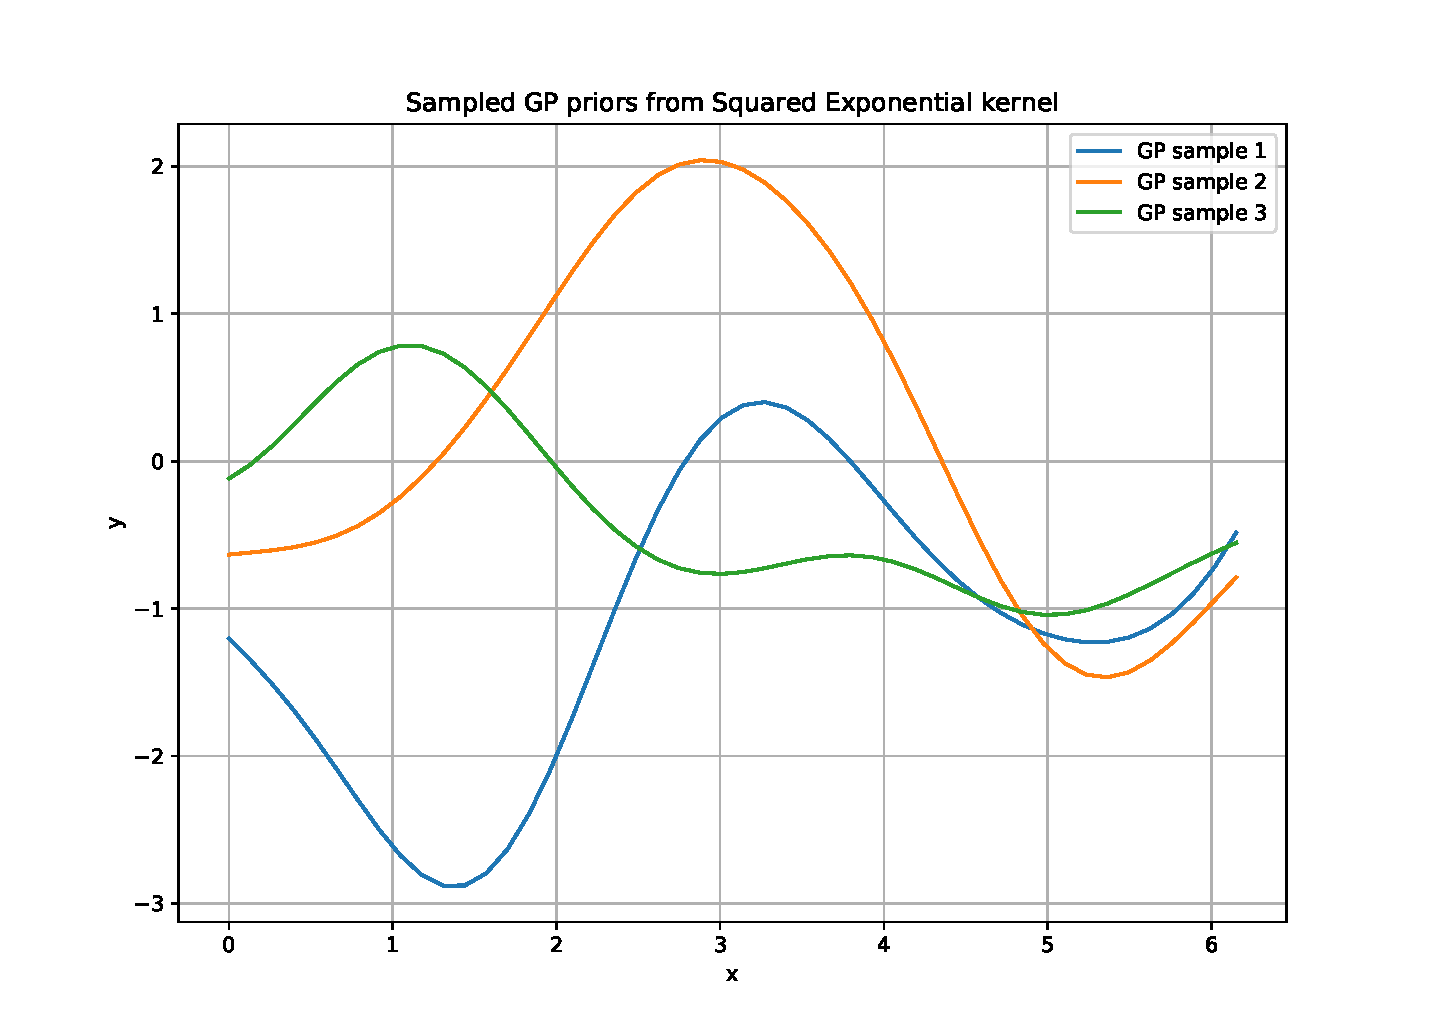
\includegraphics[width=\textwidth]{figures/chapter2/drawPrior}
\end{figure}

There's one important concept to explain before we move on. Notice in Figure \ref{fig:drawPrior} that the drawn functions seem to have a characteristic length-scale. This can be interpreted as the distance you have to move in input space before the function value changes significantly. By default, the squared exponential kernel uses a characteristic length-scale of 1 ($l = 1$). To change this behaviour to another, it is sufficient to consider $r/l$ instead of $r$ in Equation \ref{sqexp}. This can be thought as an hyperparameter to optimize, but we will return to this in another section.

\section{Prediction using a Gaussian Process prior}

This is probably the most important section in this chapter. We will learn how to incorporate the knowledge of training data $D = \left\lbrace \left(\boldsymbol{x_i}, y_i\right) | i = 1,\dots,n\right\rbrace$ into our Gaussian Process to obtain a posterior predictive distribution. We will start considering the case that we have a noiseless function, that is to say, when $\sigma^2_n = 0$. Let us define $K(X, X_{*})$, the covariance function evaluated on train and test points, $K(X, X)$ the covariance function evaluated at only the training points, $K(X_{*}, X_{*})$ equivalently defined for the test values. Notice the last two have to be square matrices by definition.\\

Let us also use the following theorem:

\begin{mydef}
\label{conditioning}
Let $\boldsymbol{x}$ and $\boldsymbol{y}$ be jointly Gaussian:
\begin{equation}
\begin{bmatrix}
\boldsymbol{x}\\
\boldsymbol{y}
\end{bmatrix} \sim N\left(
\begin{bmatrix}
\boldsymbol{\mu_x}\\
\boldsymbol{\mu_y}
\end{bmatrix},
\begin{bmatrix}
A   && C \\
C^T && B
\end{bmatrix}
\right)
\end{equation}

Then $\boldsymbol{x|y} \sim \left(\boldsymbol{\mu_x} + C B^{-1}(\boldsymbol{y} - \boldsymbol{\mu_y}), A - CB^{-1}C^T \right)$
\end{mydef}

The reader might already be guessing what we are about to do now in terms of the training output points $\boldsymbol{f}$ and the corresponding testing points $\boldsymbol{f_*}$. According to the prior chosen in \ref{fprior}, assume that $\boldsymbol{f}$ and $\boldsymbol{f_*}$ are jointly Gaussian:

\begin{equation}
\begin{bmatrix}
\boldsymbol{f}\\
\boldsymbol{f_*}
\end{bmatrix} \sim N\left(
\boldsymbol{0},
\begin{bmatrix}
K(X, X)  && K(X, X_*) \\
K(X_*, X) && K(X_*, X_*)
\end{bmatrix}
\right)
\end{equation}


We are interested now in the distribution of $\boldsymbol{f_{*}}|\boldsymbol{f}$. Simply applying Theorem \ref{conditioning}, we can obtain:

\begin{equation}
\boldsymbol{f_*|f} \sim N\left(K(X_*, X)K(X, X)^{-1}\boldsymbol{f}, K(X_*, X_*) - K(X_*, X)K(X, X)^{-1}K(X, X_*) \right)
\end{equation}

This is pretty much everything basic there is to know about Gaussian Process estimation for regression. Now we have a complete predictive distribution over test values $\boldsymbol{f_{*}}$, and we can do with it what we please. For example, one could obtain an estimate of this function by drawing samples from a multivariate normal with the computed posterior parameters, or obtain a MAP estimate using the posterior mean.\\

Let us now consider the scenario where observations are not noise-free, that is, each time you query the function there is a i.i.d Gaussian error with mean $0$ and variance $\sigma_n^2 > 0$. Assume now the following prior on the noisy observations:

\begin{equation}
Cov(\boldsymbol{y}) = K(X, X) + \sigma^2_n I 
\end{equation}

Following the exact same math as before, but taking into account this new term, we got the following joint distribution:

\begin{equation}
\begin{bmatrix}
\boldsymbol{f}\\
\boldsymbol{f_*}
\end{bmatrix} \sim N\left(
\boldsymbol{0},
\begin{bmatrix}
K(X, X) + \sigma^2_n I && K(X, X_*) \\
K(X_*, X) && K(X_*, X_*)
\end{bmatrix}
\right)
\end{equation}

And conditioning again $\boldsymbol{f_{*}}$ on $\boldsymbol{f}$, we obtain our final predictive distribution:

\begin{equation}
\boldsymbol{f_*|f} \sim N(\boldsymbol{\overline{f_*}},  Cov(\boldsymbol{f_*}))
\end{equation}

where now:

\begin{align}
\boldsymbol{\overline{f_*}} = K(X_*, X)\left(K(X, X) + \sigma^2_n I   \right)^{-1}\boldsymbol{y}\\
Cov(\boldsymbol{f_*}) = K(X_*, X_*) - K(X_*, X)\left(K(X, X) + \sigma_n^2 I \right)^{-1}K(X, X_*)
\end{align}

It will probably be useful to note that a Gaussian Process model can be written easily in terms of a Bayesian hierarchical model, since:

\begin{align}
\label{hierarchical}
\boldsymbol{y}|\boldsymbol{f} \sim N(\boldsymbol{f}, \sigma^2_n I)\\
\label{hierarchical2}
\boldsymbol{f}|X \sim N(\boldsymbol{0}, K(X, X))
\end{align}

In fact, one can also assume other priors, even over $\sigma_n^2$. This representation may help us understand the introduction of the \textit{marginal likelihood}. This marginal likelihood in a Gaussian Process setting is defined as:

\begin{equation}
p(\boldsymbol{y}|X) = \int p(\boldsymbol{y}|\boldsymbol{f}, X)p(\boldsymbol{f}|X) d\boldsymbol{f}
\end{equation}

Using the results from Equations \ref{hierarchical} and \ref{hierarchical2} we can derive the integral analitically to obtain:
\\


\chapter{Bayesian optimization}
\chapter{Experiments}
\chapter{pyGPGO: A simple Python Package for Bayesian Optimization}

\end{document}